\begin{minipage}[b]{0.65\textwidth}
\begin{Exercise}[title = rutschender Zylinder, origin = EstPho 2016, difficulty = 3, label = cylinder]
 Ein Zylinder der Masse $m$ und mit dem Radius $R$ rutscht auf einer Platte mit einer Geschwindigkeit $v$ und einer Winkelgeschwindigkeit $\omega$. Nachdem der Zylinder aufhört zu rutschen, bewegt er sich mit einer Geschwindigkeit $v$ in die entgegengesetze Richtung. Wie groß war $\omega$?
\end{Exercise}
\end{minipage}
\begin{minipage}[t]{0.35\textwidth}
	\centering
	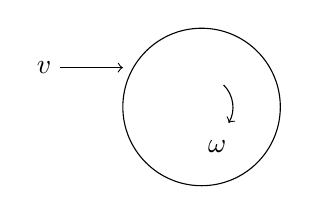
\begin{tikzpicture}
	\draw (0,0) circle (1);
	\draw[->] (-1.8,.5) -- (-1,.5);
	\node at (-2,.5) {$v$};
	\draw[->] (0.28,0.28) arc (45:-30:.4);
	\node at (.2,-.5) {$\omega$};
	\end{tikzpicture}
\end{minipage}
